\section{Literature Review} \label{sec:literature-review}

\subsection{Existing Work in AUV/ROV Docking}
Autonomous Underwater Vehicle (AUV) docking has been a focus of research for decades, driven by the need for long-duration missions via subsea battery recharging and data transfer. A wide range of docking guidance strategies  has been explored, as summarized in recent surveys \cite{yazdani2020survey}. Broadly, approaches are categorised by the sensing and guidance modality. Acoustic homing using sonar beacons can guide AUVs from long range, often providing range and bearing to a dock \cite{maire2009vision}. Electromagnetic docking systems have also been tested (e.g. using low-frequency EM fields for short-range homing), notably in Feezer's EM homing system \cite{feezor2001autonomous}. Vision-based techniques, using cameras to detect visual markers, offer high precision in final alignment. In practice, multi-modal solutions are common: for example, an AUV might navigate toward a dock via acoustic homing signals and then switch to vision-based guidance in the final meters \cite{maire2009vision}. Dedicated docking markers can be active (such as flashing lights or LED beacons) to increase visibility, or passive high-contrast patterns that require no power, as demonstrated in Marie's pole design for homing detection. On the mechanical side, most docking station designs incorporate funnel-shaped guide surfaces to help capture the vehicle despite some misalignment. This combination of sensor guidance and mechanical alignment ensures a robust docking process under various conditions.

\subsubsection{AUV Docking Demonstrations}
Numerous projects have demonstrated AUV docking with different infrastructures and homing strategies. One of the earliest was the WHOI REMUS AUV docking system from the late 1990s, which used a Relative Acoustic Tracking system of acoustic transponders for homing into a funnel-like subsea dock (see Figure~\ref{fig:remus-auv}).
\begin{figure}[H]
    \centering
    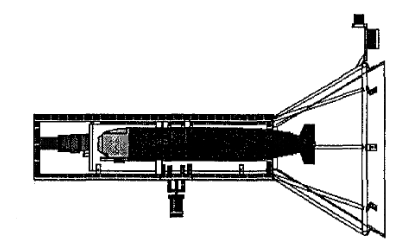
\includegraphics[width=0.6\textwidth]{Figures/remus-auv.png}
    \caption{A side-view drawing of the WHOI REMUS AUV docking system \cite{stokey1997docking}.}
    \label{fig:remus-auv}
\end{figure}

Researchers have since tested seabed-mounted and moored docking stations to support AUV missions. For instance, Maire et al. (2009) proposed a heavy weighted docking target pole lowered to the seafloor, equipped with an acoustic beacon for long-range localisation and a visual pattern for final approach. An AUV can home to such a seafloor station, attach itself, and enter a sleep or recharge mode until the next mission window.
\begin{figure}[H]
    \centering
    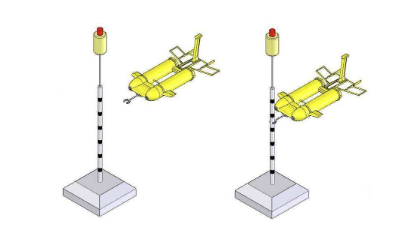
\includegraphics[width=0.6\textwidth]{Figures/maire-dock-diagram.png}
    \caption{Marie et al.'s seabed docking station concept with acoustic and visual homing aids. (left: on approach; right: after docking)\cite{maire2009vision}}
    \label{fig:maire-dock}
\end{figure}

Another notable docking system design is Trslic's moored docking station, which a cage-like docking garage was hung under a support vessel, allowing the AUV to navigate into the cage and be lifted out without surfacing on its own.
\begin{figure}[H]
    \centering
    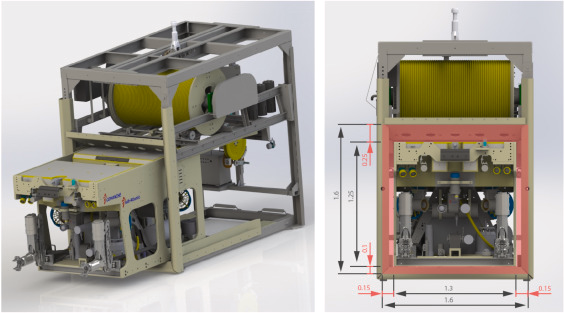
\includegraphics[width=0.6\textwidth]{Figures/trslic-dock-cage.png}

    \caption{Trslic's Tether Management System (TMS) docking cage for work-class ROVs.\cite{trslic2020vision}}
\end{figure}

\subsubsection{ROV Docking and Industrial Practice}
ROVs, being tethered and human-piloted, traditionally “dock” via their TMS rather than autonomous stations. In industry, a work-class ROV is typically deployed within a TMS, essentially an underwater cage or “garage”, that is lowered from the surface. The ROV undocks to perform its task and later returns to latch into the TMS for recovery to the ship. This process is usually manual: an ROV pilot must carefully navigate the vehicle back into the moving cage, which is task made difficult by limited visibility and the unpredictablility of the water current. To improve safety and extend operational envelopes, recent research has begun automating ROV docking. Notably, Trslic demonstrated the first autonomous TMS docking for a heavy work-class ROV in the North Atlantic (2019) \cite{trslic2020vision}. Using a vision-based pose estimation system and the four active light markers on the TMS, their ROV was able to locate and insert itself into a standard cage without any special modifications to the hardware. This trial, performed well in dynamic wave conditions, showed that autonomous control could consistently outperform human pilots for TMS docking, reducing the risk of collision and timing errors for such expensive equipment. The success of this approach is a major step toward “resident ROVs” that live subsea. In a different vein, researchers have also developed hybrid docking setups where an ROV acts as a mobile docking station to service AUVs. One such system (by Mitsubishi Heavy Industries) called Naminou equips an ROV with an electromagnetic coupling and wireless charger to capture an AUV in open water for battery charging \cite{morinaga2021development}.
\begin{figure}[H]
    \centering
    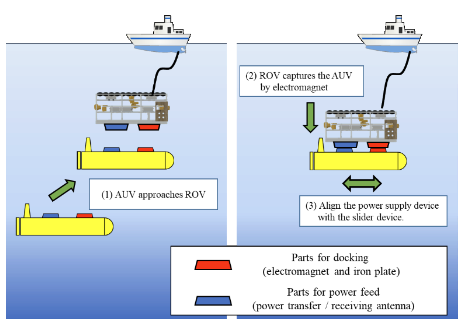
\includegraphics[width=0.6\textwidth]{Figures/morinaga-auv-flow.png}

    \caption{A flowchart of ROV-AUV docking interaction from Morinaga et al. \cite{morinaga2021development}}
    \label{fig:morinaga-auv-flow}
\end{figure}
In trials of this concept, the AUV would autonomously approach the hovering ROV using acoustic and sonar guidance, then hold position while the ROV latches onto it and aligns the power transfer coils (see Figure~\ref{fig:morinaga-auv-flow}). This illustrates the breadth of ROV-involved docking solutions, from improving launch/recovery systems to enabling ROVs as docking stations for AUV support.

\subsection{Vision-Based Docking Techniques}

Underwater docking for AUVs relies on robust computer vision methods due to the challenges of the marine environment. Vision-based techniques provide precision in final alignment and locking phase of the docking process, complementing other sensors (like acoustics) when an AUV approaches a docking station. Key approaches include using markers, active visual beacons, deep learning for target recognition, optical flow/feature tracking for motion estimation, and specialised underwater image enhancement. This section provides an in-depth analysis of these techniques and their effectiveness under underwater conditions.

\subsubsection{Existing Passive Marker-Based Docking Techniques}
\label{sec:passive-marker-docking}
Markers such as AprilTags and ArUco codes are popular for robotic navigation and pose estimation. These markers are detected by extracting the four corner verticies, followed by a Perspective-n-Point (PnP) algorithm to compute the 6-DOF pose of the marker relative to the camera. The low compuation cost and geometric accuracy make them attractive for underwater docking guidance.

Passive visual markers for underwater docking are typically high-contrast black and white patterns or coded shapes that can be reliably detected by a camera and used for pose estimation. Early work focused on designing marker geometries and classical vision pipelines that remain detectable despite turbidity, color shift and variable lighting. More recent research has extended these ideas using fiducial systems such as ArUco or AprilTag, often combined with learning-based detectors, while still relying on the geometric structure of a printed pattern for precise pose estimation.

Marie's Stagbug AUV docking system uses a binary encoded pole as a pssive black and white target mounted inside a suspended docking station. The pattern is design so that it is visible from any aribitrary yaw, roll or pitch angle and also serves as a structural station that the AUV can grip on. Detection is performed with a fast Haar feature template matcher over the image, where the 'dash-dot-dash' black and white pattern is scored over over multiple scores, position and image rotations to locate the camera pose relative to the dock \cite{maire2009vision}. As the AUV approaches closer, the system switches to shorter templates to maintaing more precise tracking at close distance. This method purely using a high contrast patten can deliver robust homing without any powered beacons, however, it is limited by the cpu cost on the template design as it searches over multiple scales and rotations, and restricts design flexibility for the dock station.

An alternate method uses common artificial fiducial markers like AprilTag and ArUco for pose estimation. Notably, Xu's AUV navigation system incorporates algorithms to detect a grid of multiple markers for improved accuracy \cite{li2015auv}. The ArUco library first decodes the marker ID and recovers each marker's pose relative to the camera. Then, Xu's custom noise model computes an optimal combined pose estimate from all visible markers, improving accuracy and robustness against individual detection errors. This work is framed for AUV navigation, but the principles apply directly to docking scenarios where multiple markers can be placed on the station for enhanced detection, as shown in Figure~\ref{fig:optical_flow}.

\begin{figure}[H]
    \centering
    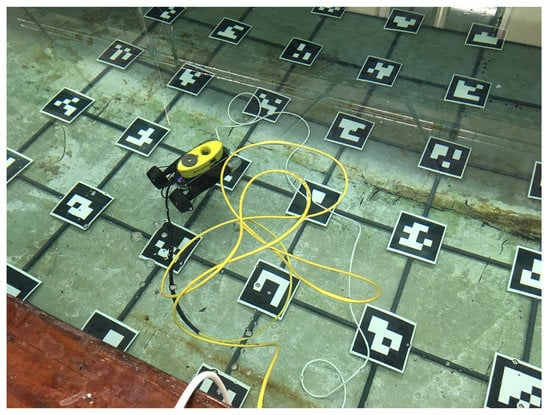
\includegraphics[width=0.6\textwidth]{Figures/xu-auv-navigration.png}

    \caption{Xu's AUV navigation test in a towing tank for camera pose estimation\cite{li2015auv}}
    \label{fig:xu-auv-navigation}
\end{figure}

Most recently, Ni et al. proposed a hybrid active and passive docking marker where a printed AprilTag is placed at the center of the dock station, surrounded by a ring of LED lights \cite{ni2025vision}, inspired by Trslic's four light beacon active marker design \cite{trslic2020vision}. A custom trained YOLO-D model is trained to simultaneously detect the LED array and the AprilTag in raw underwater images (see Figure~\ref{fig:yolo-d}).
\begin{figure}[H]
    \centering
    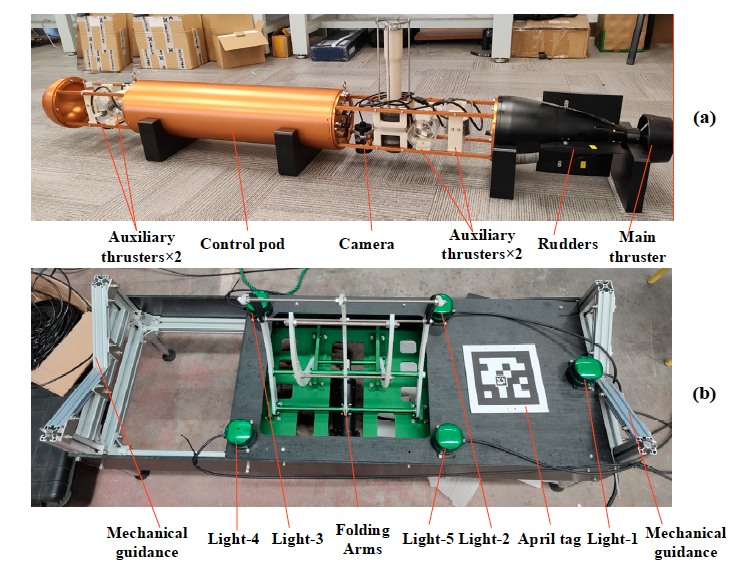
\includegraphics[width=0.6\textwidth]{Figures/msae-dock-and-auv-diagram.png}

    \caption{Example of an underwater docking station and vehicle: (a) AUV; (b) Docking station with five green LED beacons (Light-1 to Light-5), AprilTag marker at the center and v-shaped mechanical guides.\cite{ni2025vision}}
    \label{fig:optical_flow}
\end{figure}
\noindent Ni et al.'s AUV docking guidance is composed of 2 level of detection:
\begin{itemize}
    \item Level I: the LED array is used as visual markers for pose estimation. However, at close range, the light scattering can introduce errors in estimating the center of the guidance light source.
    \item Level II: the AprilTag is used for precise pose estimation. However, this guidance method is limited by the detection range and visibility of the tag under turbidity, water quality and illumination.
\end{itemize}
The docking process begins by capturing an image, which is preprocessed through configured filters to minimise noise in the image. The YOLO-D model then detects the center \(X_L\) of the LED array and the AprilTag region of interest (ROI) in the image frame. In Level I guidance, the obtained \(X_L\) is used to compute a coarse position \(P_L\) of the docking station relative to the AUV. In Level II guidance, the AprilTag corners \(X_A\) are extracted from the ROI and used to compute a precise pose \(P_A\) via PnP. Finally, the pose estimates from both levels are fused to compute overall \(P_out\), following the formula:

\[ P_{out} = w_L P_L + w_A P_A \]

where \(w_L\) and \(w_A\) are weights assigned to the Level I and Level II pose estimates based on their preconfigured confidence levels. This fusion allows the system to leverage the long-range detection of the LED array while maintaining the precision of the AprilTag when visible. The full semantic of the system is illustrated in Figure~\ref{fig:yolo-d}.

\begin{figure}[H]
    \centering
    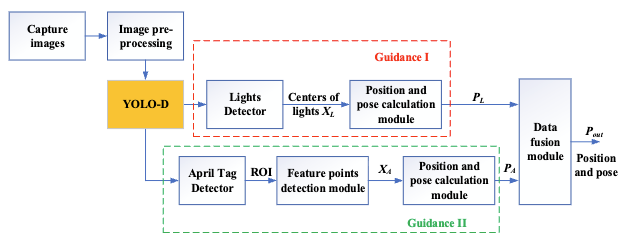
\includegraphics[width=0.7\textwidth]{Figures/msae-yolo-d-software-structure.png}
    \caption{Ni et al.'s AUV software structure for marker to pose estimation \cite{ni2025vision}. }
    \label{fig:yolo-d}
\end{figure}

These existing works show a clear evolution in passive marker-based underwater docking techniques, from simple high-contrast patterns to sophisticated multi-marker systems combining fiducials and active lights. Ealy systems like the encoded pole rely on hand-crafted patterns and feature template matching. Though their experiments demonstrated robust detection in controlled tank conditions, the computational cost and sensitivity to lighting changes limit their practical range. ArUco/AprilTage based system are able to leverage well-established libraries for detection and pose estimation, but their performance underwater can degrade due to turbidity and lighting variability. Ni et al.'s hybrid approach combining active LED markers with AprilTags through YOLO-D detection achieves higher robustness in underwater disturbances, yet trade-offs in model size, training data and onboard compute remain challenges for real-time deployment. Overall, passive marker-based docking remains a viable and effective strategy, especially when combined with active markers and learning-based detection to overcome underwater visibility challenges.

\subsubsection{Learning-Based Approaches using CNN Detection}

Modern deep learning has been a game changer for underwater vision. Instead of manually designed filters or thresholding, Convolutional Neural Networks (CNNs) can be trained to recognise the docking station or its markers in complex underwater images even under low light conditions.

A prominent trend is adapting state-of-the-art detectors like YOLO (You Only Look Once) for underwater use. These one-stage detectors are fast and can work in real time on AUV hardware. However, standard YOLO models trained on everyday images perform poorly underwater due to low-light conditions \cite{DAS20253042}. Researchers have created underwater-specific variants: for example, Pan et al.(2024) proposed YOLOv9s-UI, adding custom attention modules to better extract features in underwater scenes \cite{app14167162}. Others integrated image enhancement into the network: Wang et al.(2023) introduced a self-localisation method using "Pseudo-3D vision-inertia for AUVs" \cite{9090979} by combining a single downward camera, IMU and a depth sensor to estimate the AUV's 3D trajectory over the seabed. This is achieved by fusing visual feature tracking of the seabed with inertial and depth measurements. However, this method assumes the seafloor is locally flat and the vehicle is always at certain relative distance to the seafloor. Ni et al. (2025) introduced a specialised network called YOLO-D aimed at docking markers \cite{ni2025vision}. YOLO-D retained the fast YOLOv11 architecture but added components for small object detection at long range, such as a BiFPN (bidirectional feature pyramid) architecture for multi-scale feature fusion and an adaptive kernel convolution (AKConv) module to improve detection accuracy and efficiency on lights and AprilTag features (see Figure~\ref{fig:yolo-d-architecture}). These enhancements significantly improved the recall of tiny distant lights or partially visible tags in testing, compared to a baseline YOLO model. In pool trials, the YOLO-D could detect and locate the LED array and AprilTag in real time, providing inputs to the docking controller even under varying lighting.

\begin{figure}[H]
    \centering
    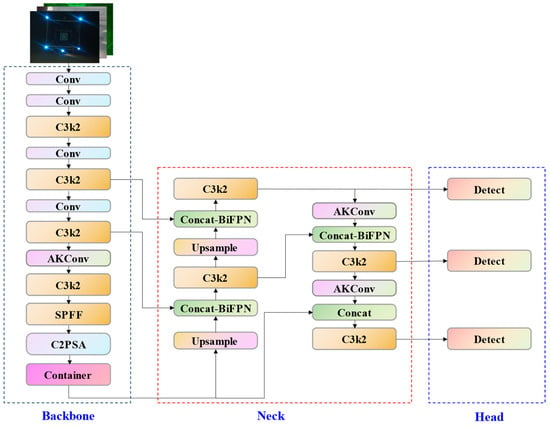
\includegraphics[width=0.7\textwidth]{Figures/yolo-d-architecture.jpg}
    \caption{Ni et al.'s YOLO-D network architecture\cite{ni2025vision}. }
    \label{fig:yolo-d-architecture}
\end{figure}

Beyond detection, some learning approaches go further by performing end-to-end control or segmentation. One innovative method used a CNN to directly output the steering command needed for docking from the camera image. Sans-Muntadas et al. (2019) tackled on the lack of underwater precise positioning systems by prosing a CNN that uses raw image from the onboard camera to estimate the heading error relative to the docking station, which is then fed to the controller to maneuver to the docking station \cite{sans2019learning}. This approach does not require explicit marker detection or pose estimation or other external sensors. However, their system produces false estimates when the dock is close to the docking station due to the lack of visible features in the close-up view.

In summary, learning-based methods (especially CNN detectors like YOLO variants) offer speed and robustness for vision-based docking. They can detect docking targets in complex scenes where classical methods fail. Yet, they often serve as part of a larger system, for example, a CNN might detect an AprilTag's bounding box, but then a precise pose is computed by a PnP algorithm on its corners. Also, pure CNN approaches for control are still experimental.

\subsection{Other Sensing Methods and Hybrid Systems}

Beyond vision, other sensing methods have been explored for underwater docking systems, including acoustic navigation, magnetic / EM homing, and mechanical alignment aids.

\subsubsection{Acoustic positioning and homing}
Acoustic based navigation system is widely used as a long range communication underwater for docking. A common configuration has an acoustic tranceiver on the dock that emits a signal, which is received by a transponder on the AUV. The AUV then replies with its own signal, allowing the dock to compute the distance based on the time delay. To obtain bearing information, several inverted ultra-short baseline (iUSBL) receivers are spaced precisely on the AUV hull. By measuring the slight time difference of arrival of the acoustic signals at each receiver, the system can triangulate the relative azimuth and elevation angles between DS and AUV. WHOI's REMUS AUV docking system is a prime example of a USBL-navigation aidded system\cite{4099107} (see Figure~\ref{fig:remus-dock} and \ref{fig:remus-dock-vehicle}). This acoustic homing can guide the AUV from long range (up to ~2km), at the cost of moderate update rates, latency due to speed of sound underwater, risk of false signals from acoustic refraction/ambient noises and limited angular resolution.

\begin{figure}[H]
    \centering
    \begin{subfigure}[b]{0.48\textwidth}
        \centering
        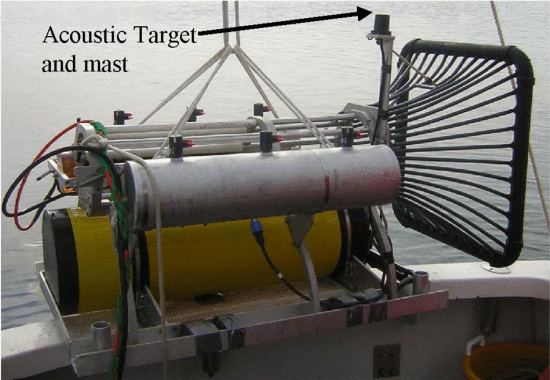
\includegraphics[width=\linewidth]{Figures/remus-dock.png}
        \caption{Remus-100 AUV docking station with labelled acoustic transceivers \cite{4099107}.}
        \label{fig:remus-dock}
    \end{subfigure}\hfill
    \begin{subfigure}[b]{0.48\textwidth}
        \centering
        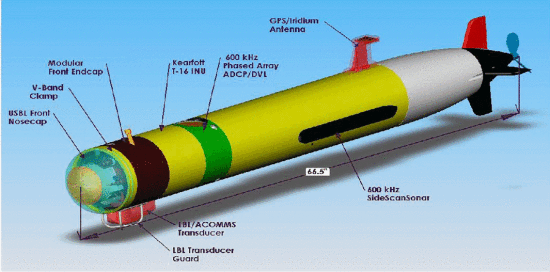
\includegraphics[width=\linewidth]{Figures/remus-docking-vehicle.png}
        \caption{Remus-100 AUV docking vehicle with labelled components. Note the USBL receivers at the nosecap \cite{4099107}.}
        \label{fig:remus-dock-vehicle}
    \end{subfigure}
    \caption{Remus-100 docking station and vehicle (left: station; right: vehicle) \cite{4099107}.}
    \label{fig:remus-dock-combined}
\end{figure}

In practice, many working-class AUVs (REMUS, Bluefin, etc.) combine iUSBL range/bearing with Doppler Velocity Logger (DVL) and inertial navigation to accomodate for current-induced drift and improve overall localisation accuracy during the approach phase.

\subsubsection{Magnetic / Electromagnetic Homing}
Electromagnetic (EM) guidance offers a more robust alternative to acoustic signal with low-frequency magnetic or electro-magnetic fields emitted by a coil on the dock, resulting in lower latency. Feezor et al. (2001) developed an EM homing system where a low-frequency magnetic field is generated by a coil on the dock, and the AUV uses magnetometers to detect the field strength and direction, without line-of-sight constraints \cite{feezor2001autonomous}. Their experiments demonstrated that the AUV could home in on the dock from a limited range up to ~30m. Further, the system requires dedicated coils, drivers and calibration of the local field environment, which may limit its practicality for general-purpose docking stations.

\subsubsection{Mechanical Alignment Aids}
Most underwater docking stations incorporate mechanical alignment aids to relax the sensing requirement and accomodate for the slight tolerances during the final docking aligment phase. There exists two main configurations: unidirectional and omnidirectional guides.

Unidirectional docking stations are the most common type of configuration, typically designed for torpedo-shaped AUVs that approach from a known heading. These stations feature funnel/cone shaped guides to help channel the vehicle into the dock despite some slight misalignment. However, this design imposes condition on the AUV to know at all time the pose of the dock relative to itself, which may not be feasible for free-floating docks as the pose and location of the dock are variables.

Omnidirectional docking stations, on the other hand, are designed to allow approach from any heading. These stations often feature a vertical structure composed of poles or cables under tension, allowing the vehicle to be latched onto the dock regardless of its orientation, notable in Odyssey IIb AUV's dock station design (see Figure~\ref{fig:oddyssey-pole-dock} and \ref{fig:oddyssey-dock-vehicle}). This design simplifies the navigation system and alignment process as the vehicle only require knowledge of the dock's location. However, omnidirectional designs requires complex mechanical design on the vehicle's nose and may not fit the requirement for all AUVs as the nose is often reserved for sensors or other equipment, and may also introduce drag on the vehicle during underwater operations.

\begin{figure}[H]
    \centering
    \begin{subfigure}[b]{0.48\textwidth}
        \centering
        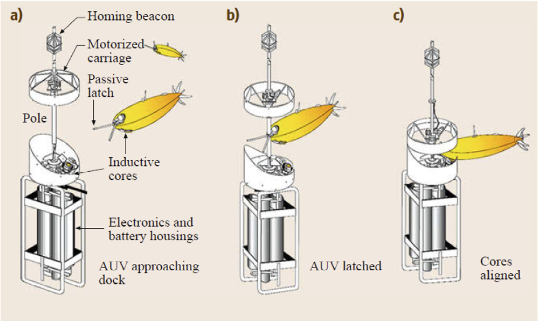
\includegraphics[width=\linewidth]{Figures/oddyssey-pole-dock.png}
        \caption{Odyssey IIb AUV docking process \cite{972084}.}
        \label{fig:oddyssey-pole-dock}
    \end{subfigure}\hfill
    \begin{subfigure}[b]{0.48\textwidth}
        \centering
        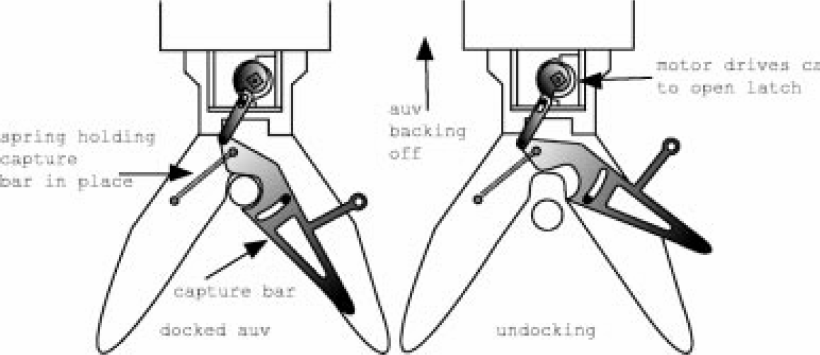
\includegraphics[width=\linewidth]{Figures/oddyssey-latch-dock.png}
        \caption{Odyssey IIb AUV latch mechanism \cite{972084}.}
        \label{fig:oddyssey-dock-vehicle}
    \end{subfigure}
    \caption{Odyssey IIb docking process and latch mechanism (left: process; right: latch mechanism) \cite{972084}.}
    \label{fig:oddyssey-dock-combined}
\end{figure}

\subsection{Addressing Known Limitations in Academic Research}

Despite substantial progress in AUV docking research, several recurring limitations appear across the literature. First, most systems assume that the docking station is either seabed-mounted or fixed in a known position and orientation. Examples include seabed poles with acoustic and visual aids \cite{maire2009vision}, fixed funnel-type garages for REMUS-class vehicles \cite{stokey1997docking}, and rigid TMS cages for work-class ROVs \cite{trslic2020vision}. In these scenarios, the dock is effectively treated as static in the world frame, and the control problem reduces to steering the vehicle into a stationary target. Free-floating platforms with their own wave-induced motion are rarely modelled explicitly, leaving a gap for docking scenarios where both the vehicle and the dock are moving bodies.

A second limitation is the experimental environment. Many vision-based docking studies are evaluated n clear-water laboratory tanks, where turbidity, backscatter, and illumination can be managed or only coarsely varied. Liu et al.'s DoNN-based cone docking, Ni et al.'s YOLO-D experiments, and various ArUco/AprilTag trials all report promising performance in tanks or test pools, but only limited results in truly turbid or highly dynamic field conditions. Quantitative evaluation across different turbidity levels, illumination levels, and camera-dock distances is often missing, making it difficult to assess how methods will perform in more challenging operational settings.

Finally, while deep learning has improved robustness in visual detection, many proposed architectures assume access to relatively powerful onboard compute and extensive labelled datasets. Underwater-specific YOLO variants, segmentation-assisted pipelines, and pseudo-3D visual-inertial systems often rely on GPU-class hardware and offline training using curated datasets. Real-time adaptation to changing turbidity or lighting is usually handled via static data augmentation or preconfigured enhancement modules rather than closed-loop adaptation. Likewise, few studies explicitly address the constraints of small or mid-size ROV hardware, where power, compute and communication bandwidth are more limited.

\subsection{How This Project Fits Into the Literature}

This project is positioned to address several of the above gaps by focusing on a vision-based docking system for a low cost ROV approaching a free-floating underwater dock. Unlike many prior works that assume a rigid, seabed-mounted or fixed-frame dock, the proposed system will explicitly consider a docking station that is suspended in the water column and mechanically coupled to a ridgid structure. This introduces relative motion between the dock and the ROV, even when both attempt to hold position, and more closely reflects resident ROV scenarios and practical offshore deployments.

On the perception side, the project builds directly on fiducial-based and learning-based detection approaches identified in the literature review. The dock will be equipped with passive markers (e.g., AprilTags or ArUco patterns) and simple active LEDs, enabling comparison between classical marker detection and lightweight CNN-based detectors inspired by recent Ni et al.'s underwater docking work. Rather than attempting to reproduce full-scale architectures such as YOLO-D, the emphasis will be on achieving robust detection and pose estimation within the compute envelope of an ROV platform, and on characterising how performance degrades under changes in turbidity, lighting and relative orientation.

Experimentally, the project aims to bridge the gap between idealised tank tests and more realistic field-like conditions. Controlled experiments will be conducted in a test environment where water clarity, lighting and dock motion can be varied in a repeatable way. Key evaluation metrics will include marker detection rate, pose estimation error, docking success rate, and latency from image capture to control command. By systematically varying environmental and hardware parameters, the project will generate practical guidelines on marker design, placement, and algorithm selection for ROV docking.

In summary, this thesis contributes to the docking literature by formulating and tackling the problem of vision-based docking to a free-floating underwater dock, tailoring and evaluating fiducial and learning-based perception methods for ROV-class hardware and constraints, and providing experimental evidence and design recommendations that help translate academic docking techniques into more realistic ROV deployment scenarios.